\documentclass[12pt]{article}

% Specify how big is going to be the paper margins.
\usepackage[a4paper, margin=1in]{geometry}

% amsmath: Add useful commans like aligh and gather.
% amsfonts: Add useful fonts like \mathbb{R}.
% amssymb: Add useful symbles like \therefore (needs amsfonts to work).
\usepackage{amsmath, amsfonts, amssymb}

% Makes the use of colors possible.
\usepackage{xcolor}

\definecolor{color1}{HTML}{084a8c}
\definecolor{color2}{HTML}{487fb7}
\definecolor{color3}{HTML}{95b7da}
\definecolor{color4}{HTML}{c9daea}

% Add Latin Modern Fonts like Sans-serif and Roman.
\usepackage{lmodern}

% Makes header and footer configurable.
\usepackage{fancyhdr}

% Makes the use of colored and configured tables possible
\usepackage{tcolorbox}

% Add commands to specify theorems like \newtheorem{x}{y}.
\usepackage{amsthm}

% Enables enumeration of items.
\usepackage{enumitem}

% Enables adding images.
\usepackage{graphicx}

% Enables cool hyper references.
\usepackage[colorlinks=true, linkcolor=color2, urlcolor=color2, citecolor=color2]{hyperref}

\title{\sffamily\bfseries{Soluções Jacob Palis 2025 N2}}
\author{Samuel de Araújo Brandão}
\date{4 de Setembro de 2025}

\pagestyle{fancy}
\fancyhf{}

\fancyhead[L]{\sffamily\bfseries{Soluções Jacob Palis 2025 N2}}
\fancyhead[R]{\textcolor{color2}{Samuel Brandão}, 4 de Setembro de 2025}
\fancyfoot[C]{\thepage}
\setlength{\headheight}{14.5pt}

\tcbset{
  statementbox/.style = {
    enhanced,
    width=\textwidth,

    title={Enunciado},
    titlefilled,
    fonttitle=\sffamily\bfseries,
    coltitle=color4
    colbacktitle=color1,

    colback=white,
    colframe=color1,
    boxrule=1pt,
    arc=2mm,
    boxsep=2pt,
  }
}

\tcbset{
  theorembox/.style = {
    enhanced,
    width=\textwidth,

    colback=white,
    colframe=color1,
    boxrule=1pt,
    arc=2mm,
    boxsep=2pt
  }
}

\tcbset{
  lemmabox/.style = {
    enhanced,
    width=\textwidth,

    colback=white,
    colframe=color2,
    boxrule=1pt,
    arc=2mm,
    boxsep=2pt
  }
}

\renewcommand*\contentsname{\textsf{Conteúdos}}
\newcommand{\kb}[1]{\left\lfloor #1 \right\rfloor}

\begin{document}
  \maketitle
  Uma coleção de soluções para a \textbf{Jacob Palis 2025 Nível 2}, inspirada no estilo de Evan Chen.
  Pode-se encontrar todos os problemas e respostas oficiais 
  \textbf{\href{https://www.obm.org.br/content/uploads/2025/06/provas_jacob_palis_2025.pdf}{aqui}}.

  Todas as soluções foram inteiramente escritas por mim, enquanto me preparava para a
  International Mathematical Olympiad (IMO).

  Caso encontre algum erro ou tiver sugestões ou comentários, sinta-se a vontade 
  para entrar em contato!

  \tableofcontents

  \clearpage

  \section{\textsf{Problemas}}
    \subsection{Testes}
      \begin{enumerate}[label=\textbf{\arabic*.}]
        \item No dia 08/06/2025, se uma pessoa somar sua idade e o ano do seu nascimento, o resultado será
        \item Lucas acompanha os preços de cartas colecionáveis numa loja online. Certo dia a carta especial custava V reais. No dia seguinte 
          o preço da mesma carta teve um aumento de P\% e passou a custar \(V + \tfrac{P}{2}\) reais. Qual é o valor de \(V\)?
        \item Um número é dito “grandinho” quando pelo menos um dos seus algarismos é maior ou igual a 5. Por exemplo, 99, 50 e 25 são 
          grandinhos, mas 20 e 13 não são. Existem quantos números grandinhos de dois algarismos?
        \item Os pontos A, B, E e H estão sobre uma reta. Do mesmo lado dessa reta são construídos os quadrados ABCD, BEFG e EHIJ com lados
          1, 2 e 3, respectivamente. Qual é a área do triângulo ACI?
          \begin{figure}[h]
            \centering
            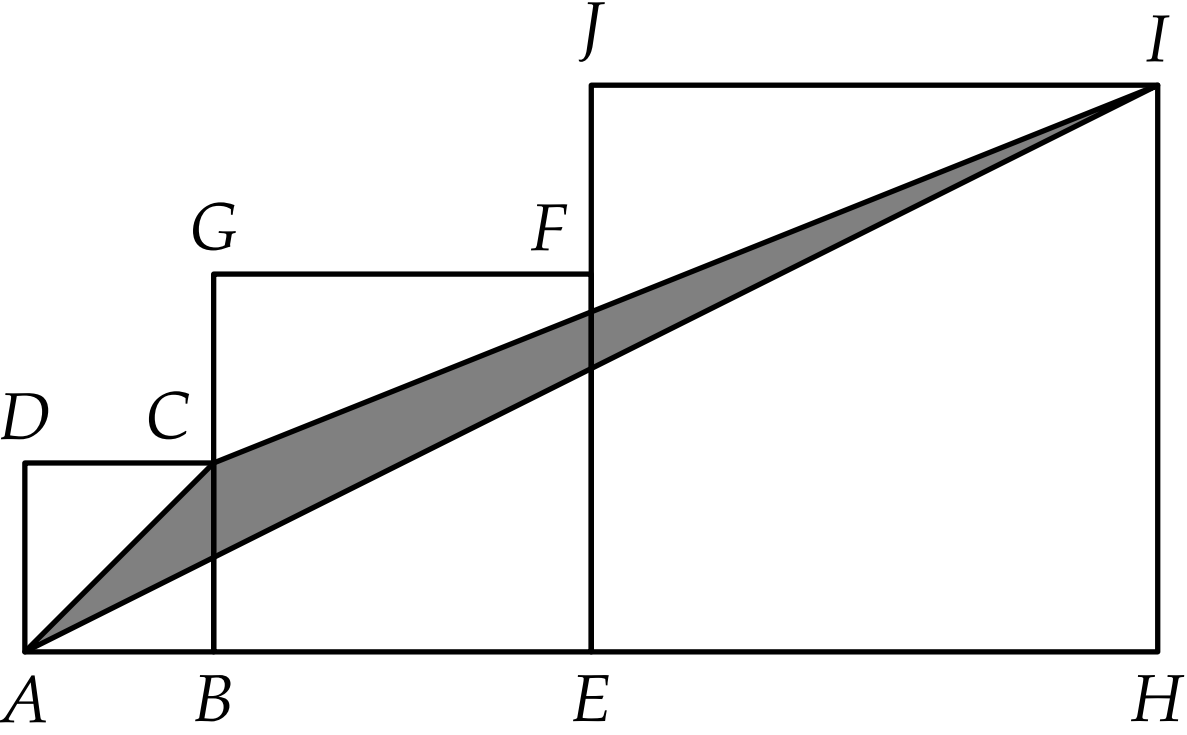
\includegraphics[width=0.4\textwidth]{first.png}
          \end{figure}
        \item Diamantino nasceu no ano 19AB, em que A e B são algarismos. Sua filha Rubi nasceu em 20CD, em que C e D são algarismos. Se
          Diamantino tivesse nascido em 19CD e Rubi tivesse nascido em 20AB, a diferença entre os dois anos de nascimento seria sete vezes a
          diferença entre os dois anos de nascimento verdadeiros. A diferença entre os anos de nascimento verdadeiros é
        \item A figura abaixo representa o mapa do Reino Estrelado. As bolinhas representam cidades e as ligações representam estradas entre 
          as cidades. Um conjunto de cidades é chamado independente se não existem duas cidades pertencentes a ele que estejam conectadas por 
          uma estrada. Qual é o número máximo de cidades que um conjunto independente no Reino Estrelado pode ter?
          \begin{figure}[h]
            \centering
            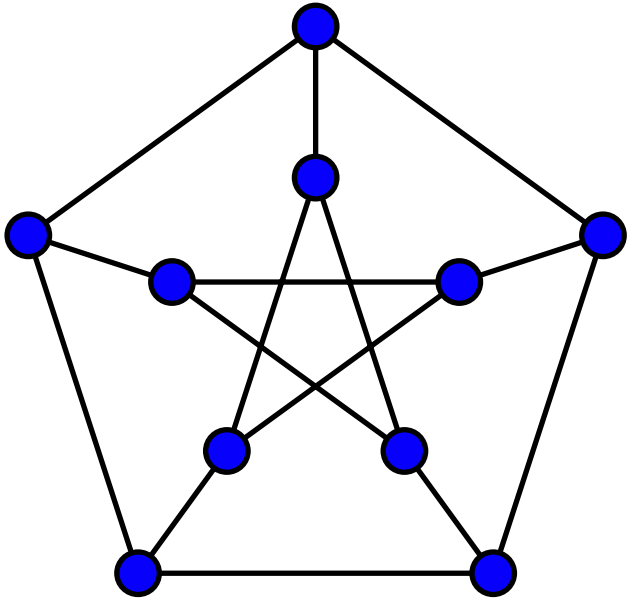
\includegraphics[width=0.3\textwidth]{second.png}
          \end{figure}
        \item Sabemos que o conjunto de números \(\{a, b, c\}\) é igual ao conjunto \(\{1, 2, 3\}\), mas não sabemos qual letra é cada número.
          Sobre os números \(a+b+c\), \(ab+c\) e \(abc\) podemos afirmar que
        \item A figura a seguir mostra um pentágono regular ABCDE, um triângulo equilátero ABF e um quadrado DGHI. Sabe-se que o ponto F está
          sobre o lado HI. Qual é a medida em graus do ângulo \(\angle AFH\)?
          \begin{figure}[h]
            \centering
            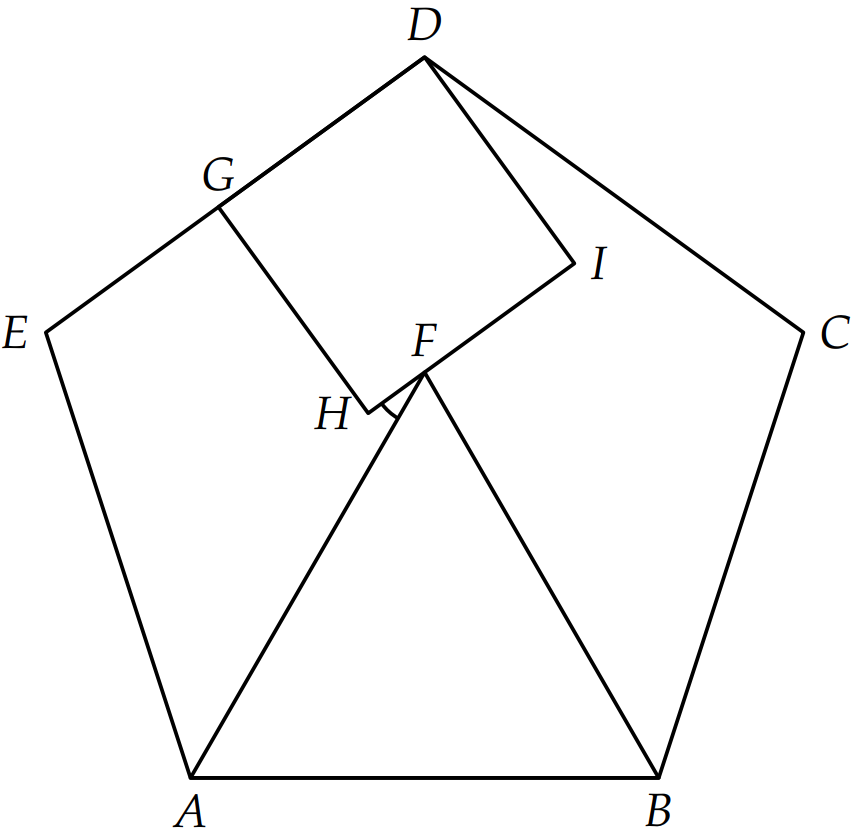
\includegraphics[width=0.4\textwidth]{third.png}
          \end{figure}
        \item Seja A um subconjunto do conjunto \(\{1, 2, 3, \dots, 10\}\) de modo que não existem dois elementos \(a\) e \(b\) de A tal
          que a diferença \(a-b\) seja um número primo. Qual é o número máximo de elementos que o conjunto A pode ter?
        \item Na figura a seguir uma circunferência de centro A passa pelos pontos B, C, D e E. O ponto A é o ponto médio de CE. A 
          circunferência de centro D que passa por E e a circunferência de centro C que passa por E se encontram novamente no ponto F
          diferente de E. Sabendo que os triângulos ABC e ACD são equiláteros, qual é a medida do ângulo \(\angle EFB\) em graus?
          \begin{figure}[h]
            \centering
            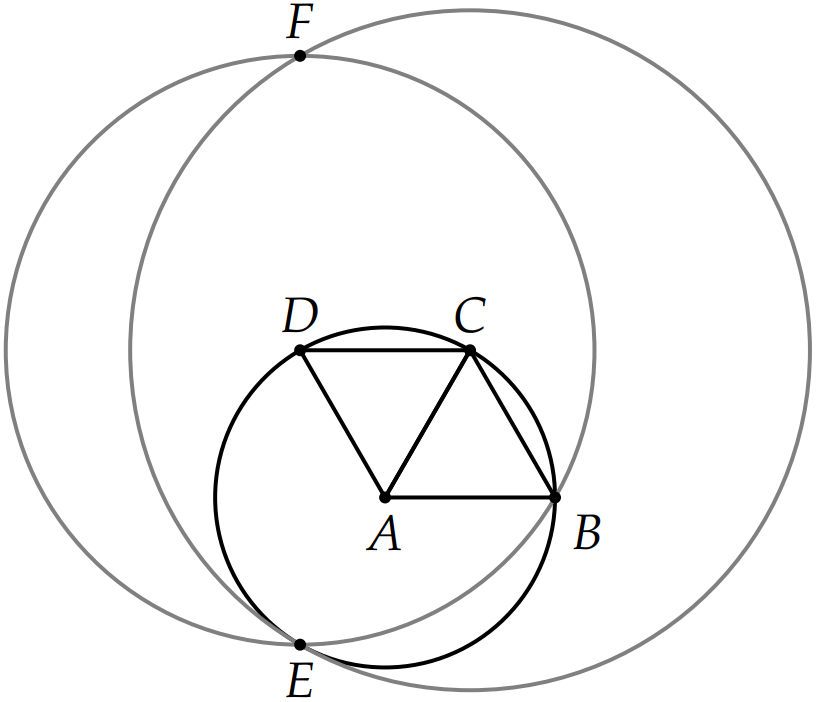
\includegraphics[width=0.3\textwidth]{fourth.png}
          \end{figure}
        \item Qual é o menor inteiro positivo \(n \geq 3\) tal que se girarmos um polígono regular P de n lados 2025º em torno do seu centro
          obtemos um polígono regular \(P'\) com vértices nas mesmas posições de P?
        \item Os reais não nulos \(a\) e \(b\) são raízes da equação \(x^2 - (a^2-b^2)x + a^2b^2 = 0\). Se \(a > b > 0\), o valor de
          \(a^3+b^3\) é

        \item Na figura a seguir, ABC, CDE e AEF são triângulos equiláteros, com C sobre o segmento BD. O ponto O é o centro do triângulo AEF.
          A medida do ângulo \(\angle ACO\)

          \begin{figure}[h]
            \centering
            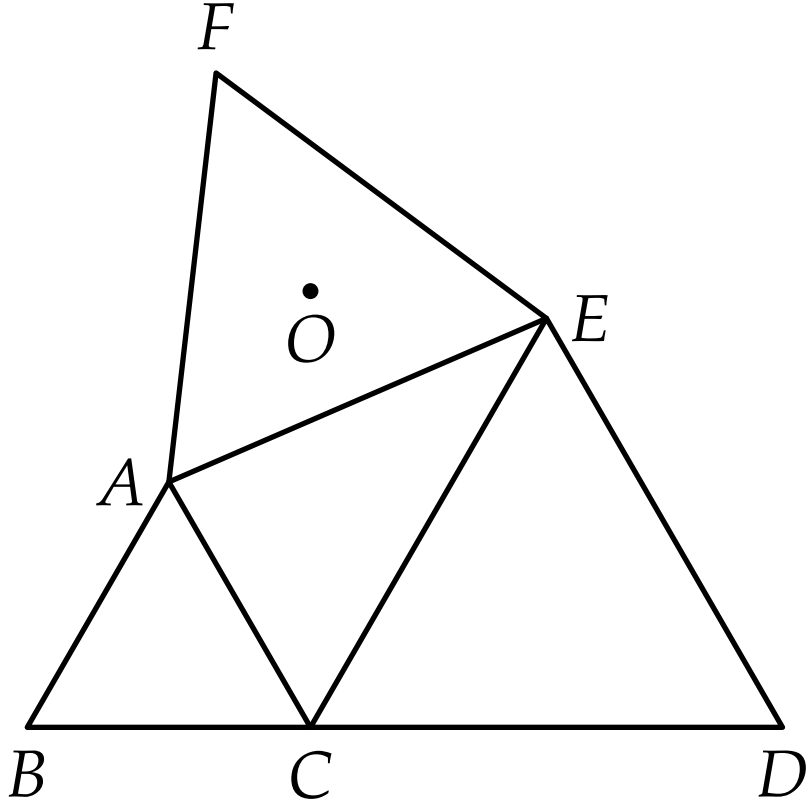
\includegraphics[width=0.3\textwidth]{fifth.png}
          \end{figure}

        \item Quantos divisores positivos de \(2025 \cdot 2520\) são múltiplos de 2025 ou de 2520?
        \item Esmeralda escreve na casa na linha \(m\) e coluna \(n\) de um tabuleiro \(201 \times 201\) o produto \(m \cdot n\). O tabuleiro 
          é pintado como no xadrez, de preto e branco. Esmeralda soma os números nas casas brancas, obtendo B, e soma os números nas casas
          pretas, obtendo P. A diferença, em módulo, entre P e B, é
      \end{enumerate}
    \subsection{Respostas Numéricas}
      \begin{enumerate}[label=\textbf{\arabic*.}, start=16]
        \item O professor Reginaldo gosta de se exercitar na esteira. Certo dia ele decidiu correr 3,5 km com velocidade de 10 km/h. Durante a corrida o painel mostra 
          8 algarismos, os primeiros 4 algarismos \(K_1K_2,V_1V_2\) indicam a distância percorrida em quilômetros com duas casas depois da vírgula (no começo mostra 00,00) e os outros
          4 algarismos indicam \(X_1X_2:Y_1Y_2\), os minutos e segundos que faltam para o professor terminar sua corrida (no final deve mostrar 00:00). Em certo momento o professor
          percebeu que os primeiros 4 algarismos ficaram exatamente iguais aos 4 últimos (o primeiro algarismo igual ao quinto, o segundo igual ao sexto e assim por diante). Nesse
          momento a soma de todos os 8 algarismos era igual a quanto?
        \item Certo inteiro positivo n tem dois algarismos. O algarismo das dezenas é \(a\), e o das unidades é \(b\). Sabe-se que \(n = b^3 - 2a\). Qual é a soma dos possíveis
          valores de n?
        \item Dizemos que dois números estão conectados se é possível ir de um para o outro somando dois algarismos consecutivos de um deles e trocando pelo resultado, mantendo
          os demais algarismos como estão. Por exemplo, 206 e 2015 estão conectados, pois podemos trocar 15 por 6 = 1+5, e 2078 e 2015 também estão conectados, pois podemos trocar
          78 por 15 = 7+8. Dizemos que dois números estão ligados se é possível ir de um até o outro usando zero ou mais números conectados intermediários. Por exemplo, 206 e 2078
          estão ligados, pois podemos usar 2015 como intermediário. Quantos números de 1 a 2025 são ligados ao 2025 (incluindo ele mesmo)?
        \item O produto de 2025 inteiros positivos é \(2025^k\), para algum k inteiro positivo. Sabe-se que nenhum dos 2025 inteiros é igual a 1. Qual é o menor valor possível de k?
        \item Seja PABCD um pentágono inscritível com \(\angle APB = \angle BPC = \angle CPD\). Além disso, sabe-se que PA = 9, PB = 15 e PC = 16. Se o valor de PD pode ser escrito
          na forma \(\tfrac{p}{q}\) com p e q inteiros positivos primos entre si, determine o valor de \(p+q\).
      \end{enumerate}
  \clearpage

  \section{\textsf{Soluções}}
    \subsection{Testes}
    \subsection{Respostas Numéricas}

  \clearpage

  \section{\textsf{Referências}}
\end{document}
